\chapter{Balanced Clustering} 

In this chapter, we examine the reasons that cause load imbalance in task clustering. Furthermore, we propose a series of task balancing methods to address these imbalance problems. A trace-based simulation shows our methods can significantly improve the runtime performance (the speedup is up to 1.4) of a widely used physics workflow compared to the naive implementation of task clustering.

\section{Motivation}


Existing task clustering strategies have demonstrated their effect in some scientific workflows such as CyberShake \cite{Rynge2012} and LIGO \cite{Deelman2002}. However, there are several challenges that are not yet addressed. 

The first challenge users face when executing workflows is task runtime variation. Tasks may have diverse task runtimes and such diversity may cause some load imbalance. The last completed task among a given set of tasks essentially controls the release of next set of tasks. 

The second challenge has to do with the complex data dependencies within a workflow. Merging tasks that have no intermediate data between them seems safe at the first sight. However, the subsequent tasks that rely on the output data that their parent tasks produce may suffer a data locality problem since data may be distributed poorly and the data transfer time is increased. 

We generalize these two challenges (Runtime Imbalance and Dependency Imbalance) to the general imbalance problem. It means that the execution of workflows suffers from significant overheads (unavailable data, overloaded resources, or system constraints) due to inappropriate task clustering and job execution. To solve the imbalance problem, we introduce a series of balancing methods to address these two challenges respectively. 

However, what makes this problem challenging is that the solutions are usually conflicting. For example, balancing runtime may worsen the Dependency Imbalance problem, and vice versa. A quantitative measurement of workflow characteristics is required to serve as a criterion to select and balance these solutions. To achieve this goal, we propose four metrics to reflect the internal structure (in terms of runtime and dependency) of the workflow. 

In particular, we provide a novel approach to capture these metrics. Traditionally, there are two approaches to improve the performance of task clustering. The first one is a top-down approach \cite{Integration2012} that represents the clustering problem as a global optimization problem and aims to minimize the overall runtime of a workflow. However, the complexity of solving such an optimization problem does not scale well. The second one is a bottom-up approach \cite{Muthuvelu2005}\cite{Liu2009} that only examines free tasks to be merged and optimizes the clustering results locally. In contrast, our work extends these solutions to consider the neighboring tasks including siblings, parents, children and so on because such a family of tasks has strong connections between them. 

%The third contribution we make is that we analyze and connect the performance of these metrics and balancing methods. These quantitative metrics indicate which type of imbalance problem a workflow is more likely to suffer from. Comparing the relative values of these metrics informs the selection of a balancing method or a combination of these methods. 

\section{Related Work}

A plethora of balanced task scheduling algorithms have been developed in the networking and OS domains \cite{Lifflander2012, Zheng2011}. Many of these schedulers have been extended to the hierarchical setting. Lifflander et al. \cite{Lifflander2012} proposed to use work stealing and a hierarchical persistence-based rebalancing algorithm to address the imbalance problem in scheduling. Zheng et al. \cite{Zheng2011} presented an automatic hierarchical load balancing method that overcomes the scalability challenges of centralized services and poor solutions of traditional distributed services. A popular technique in workload studies  to address the load balancing challenge is overdecomposition \cite{Lifflander2012}. This method decomposes computational work into medium-grained tasks. Each task is coarse-grained enough to enable efficient execution and reduce scheduling overheads, while being fine-grained enough to expose significantly higher application-level parallelism than that is offered by the hardware. In comparison, our work aims to create clustered jobs that have an even distribution in both job runtime and dependency. The reason is that workflows usually have multiple execution levels and the load balance in each level has an influence on the load balance problem in other levels. We distinguish our work by introducing a quantitative approach to measure the imbalance problem in a workflow and then guide the selection of different balanced task clustering methods. 


Park et al. \cite{Humphrey2008} limits the amount of parallel data transfer to avoid overloading supporting services such as data servers, which is called data throttling. Throttling is especially useful for unbalanced workflows in which one task might be idle while waiting for data to arrive. However, as discussed in \cite{Humphrey2008}, data throttling has an impact on the overall workflow performance depending on the ratio between computational and data transfer tasks. Therefore, performance analysis is necessary after the profiling of data transfers so that the relationship between computation and data transfers can be identified more explicitly. Rodríguez \cite{Rodríguez2012} proposed an automated and trace-based workflow structural analysis method for DAGs. Files transfers are accomplished as fast as the network bandwidth allows, and once transferred, the files are buffered/stored at their destination. To improve the use of network bandwidth and buffer/storage within a workflow, they adjusted the speeds of some data transfers and assured that tasks have all their input data arriving at the same time. Compared to our work, data throttling has a limit in performance gain by the amount of data transfer that can be reduced, while our partitioning approach can improve the overall workflow runtime and resource usage. 

With the aim of dynamically balancing the computational load among resources, some jobs have to be moved from one resource to another and/or from one period of time to another, which is called task reallocation \cite{Tomas2012}. Caniou  \cite{Caniou2011} presented a reallocation mechanism that tunes parallel jobs each time they are submitted to the local resource manager (which implies also each time a job is migrated). They only needed to query batch schedulers with simple submission or cancellation requests.  Its authors also presented different reallocation algorithms and studied their behaviors in the case of a multi-cluster Grid environment. In \cite{Zhang2000}, a pre-emptive process migration method was proposed to dynamically migrate processes from overloaded nodes to lightly-loaded nodes. However, it can achieve a good balance only when there are some idle compute nodes (e.g. when the number of task processes is less than that of compute nodes). In our case with large scale scientific workflows, usually we have more tasks than available compute nodes . 

Guo et al. \cite{Zhenhua2011} presented mechanisms to dynamically split and consolidate tasks to cope with load balancing and break through the concurrency limit resulting from fixed task granularity. They have proposed algorithms to address the load balancing problem in single-job systems and prior knowledge is not required. For multi-job cases, they used a shortest-job-first algorithm to minimize job turnaround time when combined with task splitting. Similarly, Ying et al. \cite{Ying2009} proposed a load-balancing algorithm based on collaborative task clustering. The algorithm divides the collaborative computing tasks into subtasks and then dynamically allocates them to the servers. Compared to these approaches, our work selects tasks to be merged based on their task runtime distribution and their data dependencies initially, without introducing additional overheads during the runtime. Also, a quantitative approach of imbalance measurement provides us a general view of multiple workflow instances with different runtime characteristics. 



\section{Approach}



\begin{figure}[!lh]
\centering

 \includegraphics[width=0.6\linewidth]{figures/balance/hc.png}
  \captionof{figure}{Task Clustering}
  \label{fig:hc}
\end{figure}


With o-DAG model, we can explicitly express the process of task clustering. For example, in Fig~\ref{fig:hc}, two tasks $t_1$ and $t_2$ without data dependency between them are merged into a clustered job $j_1$. Scheduling overheads ($s$) are reduced but clustering delay is added. After horizontal clustering, $t_1$ and $t_2$ in $j_1$ can be executed in sequence or in parallel if supported. In this work, they are executed in sequence. Given one available resource, the overall runtime for the workflow (left) is $runtime_1=s_1+t_1+s_2+t_2$ , and the overall runtime for the workflow (right) is $runtime_2=s_1+c_1+t_1+t_2$.  $runtime_1>runtime_2$ as long as  $c_1<s_2$ which is true in many distributed systems since the clustering delay within a worker node is usually smaller than the scheduling overhead across different worker nodes.  

%\textbf{Task Clustering}  is an optimization technique that merges fine-grained tasks into larger jobs to reduce the scheduling overhead and thereby the overall runtime is reduced as well. Specifically, Pegasus WMS \cite{Singh2008} supports horizontal clustering and label-based clustering. \textbf{Horizontal Clustering} (HC) merges tasks on the same level of the workflow. In their work, the level for a task is determined by doing a Breadth First Search of the underlying DAG. In contrast, we define the level of a task as the longest depth from the root task to this task (Depth First Search) because the longest depth controls the final release of this task. In label-based clustering, the user identifies tasks in the abstract workflow description that they want to execute as one cluster by associating labels with the tasks. Tasks associated with the same label are put into the same clustered job. However, these techniques are not aware of the data dependencies and expected runtime of tasks. 

\begin{figure}
\centering
  \includegraphics[height=0.4\linewidth]{figures/balance/vc.png}
  \captionof{figure}{Vertical Clustering}
  \label{fig:vc}
\end{figure}



Fig~\ref{fig:hc} shows a typical example of \textbf{Horizontal Clustering} (HC) that merges tasks at the same horizontal level. In our work, we define the level of a task as the longest depth from the root task to this task (Depth First Search) because the longest depth controls the final release of this task. Fig~\ref{fig:vc} shows another type of clustering called \textbf{Vertical Clustering} (VC) that aims to merge tasks at the same pipeline. A pipeline of tasks is a chain of tasks (such as $t_1$, $t_5$ and $t_9$ in Fig~\ref{fig:pipeline}) connected by data dependencies. Particularly any two connected tasks in a pipeline should have a one-to-one relationship, which means the parent task is the only parent of the children task and the children task is the only children of the parent task. 

In conclusion, the o-DAG allows a high level of details in specification of the system overheads and it is more powerful than the DAG model in the case of task clustering.
% used in some previous work. 




%Figure 9 shows how we implement VC. Once we detect there exist a one-to-one relationship between two tasks (line 5), we merge them. Below we prove that VC is always beneficial and thereby it is always safe to perform VC. In Figure 10, $t_1$ is a parent of $t_2$ and VC merges them into a new job $j_1$. The overall makespan of the two tasks before clustering is $runtime_1=s_1+t_1+s_2+t_2$, and the overall makespan after clustering is $runtime_2=s_1+c_1+t_1+t_2$. 
%Similar to the discussion in Figure 3, we conclude that it is always beneficial (but not necessarily optimal) to perform vertical clustering because it may cause other imbalance problems to be shown below. VC is particularly useful when we have a Runtime Imbalance problem caused by dependencies with offspring tasks since we can merge tasks at the same pipeline and this problem is simplified to the Runtime Imbalance problem caused by child tasks. 

\subsection{Balanced Clustering Metrics}


As already mentioned, in this work, we discuss two imbalance problems:



\textbf{Runtime Imbalance} describes the difference of the task runtime of a group of tasks. Among all the types of Runtime Imbalance, we use two basic ones: \textbf{Horizontal Runtime Variance} ({\em HRV}) and \textbf{Pipeline Runtime Variance} ({\em PRV}). {\em HRV} is defined as the standard deviation of task/job runtime at the same horizontal level. At the same horizontal level, the job with the longest runtime often controls the release of next level jobs. 


\begin{figure}

\centering
  \includegraphics[width=0.5\linewidth]{figures/balance/rv.png}
  \captionof{figure}{Runtime Variance}
  \label{fig:rv}
\end{figure}
\begin{figure}
\centering
  \includegraphics[width=0.3\linewidth]{figures/balance/pipeline.png}
  \captionof{figure}{Pipelines}
  \label{fig:pipeline}
\end{figure}



Therefore, to improve the runtime performance, it is meaningful to reduce the standard deviation of job runtime. Fig~\ref{fig:rv} shows a simple example with four independent tasks ($t_1$, $t_2$, $t_3$ and $t_4$) while the task runtime of $t_1$ and $t_2$ is half of that of $t_3$ and $t_4$. In the naive approach of Horizontal Clustering (HC), a possible clustering result could be merging $t_1$ and $t_2$ as a job and $t_3$ and $t_4$ as the other job, which creates two clustered jobs with different job runtime. In contrast, a balanced clustering strategy should try its best to evenly distribute task runtime among jobs as Fig~\ref{fig:rv} (bottom) shows. Generally speaking, a smaller Horizontal Runtime Variance ({\em HRV}) means that the runtime of tasks at the same horizontal level is more evenly distributed and therefore it is less necessary to balance the runtime distribution. 
%For example, the {\em HRV} of the first level tasks in Fig~\ref{fig:dv} is the standard deviation of $t_1$, $t_2$, $t_3$, and $t_4$. 


Pipeline Runtime Variance ({\em PRV}) is defined as the standard deviation of the cumulative runtime of pipelines. For example, the {\em PRV} of the four pipelines in Fig~\ref{fig:pipeline} is the standard deviation of ($t_1+ t_5 +t_9$), ($t_2+t_6+t_{10}$), ($t_3 +t_7+t_{11}$), and ($t_4+t_8+t_{12}$).

%is the second reason why we need to use balanced clustering and it

\begin{figure}
\centering

  \includegraphics[width=0.8\linewidth]{figures/balance/dv.png}
  \captionof{figure}{Dependency Variance}
  \label{fig:dv}
\end{figure}
\textbf{Dependency Imbalance} means that the task clustering at one horizontal level forces the tasks at the next level (or even next few levels) to have severe data locality problem and thus a reduction in parallelism exists. For example, in Fig~\ref{fig:dv}, we show a workflow with two levels of tasks. Merging $t_1$ and $t_2$ together and $t_3$ and $t_4$ together forces $t_5$ and $t_6$ to transfer files from two locations and $t_5$ and $t_6$ have to wait until the completion of $t_1$, $t_2$, $t_3$, and $t_4$.  While a balanced clustering strategy should try to merge tasks that share child tasks together as much as possible and $t_5$ can start to execute once $t_1$, $t_2$ are completed and so can $t_6$. To measure and demonstrate the Dependency Imbalance of a workflow quantitatively, we propose two types of metrics below. 



We first define the \textbf{Impact Factor} ($IF$) of a task in a recursive way as below. 

\begin{equation}
 IF(t_u)=\sum_{t_v\in Child(t_u)}^{}\frac{IF(t_v)}{L(t_v)}
\end{equation}
where $Child(t_u)$ indicates the set of child tasks that task $t_u$ has and $L(t_v)$ is the number of parents task $t_v$ has. For simplicity, we assume the $IF$ of the exit task of a workflow is 1.0 such as $t_7$ in Fig~\ref{fig:hifv}. Given a workflow in Fig~\ref{fig:hifv} (Left), we show the $IF$ of these tasks:
\begin{eqnarray}
\displaystyle  
&IF(t_7 )=1.0, IF(t_6 )=IF(t_5 )=IF(t_7 )/2=0.5\nonumber  \\
&IF(t_1 )=IF(t_2 )=IF(t_5 )/2=0.25,IF(t_3 )=IF(t_4 )=IF(t_6 )/2=0.25\nonumber 
\end{eqnarray}


\begin{figure}
\centering
  \includegraphics[width=0.8\linewidth]{figures/balance/hifv.png}
  \captionof{figure}{An Example of HIFV and HDV}
  \label{fig:hifv}
\end{figure}


Runtime variance is not able to describe how `evenly' or `disordered' dependencies are distributed among tasks. In Fig~\ref{fig:hifv}, the left workflow should have a smaller Dependency Imbalance problem than the right workflow since the dependencies in the left figure are more repetitive and regular. We define the \textbf{Impact Factor Variance} ({\em IFV}) of tasks to be the standard deviation of their $IF$. Therefore, the {\em IFV} of {$t_1$, $t_2$, $t_3$, $t_4$} is 0. In contrast, for the workflow in Fig~\ref{fig:hifv} (Right), we have:
\begin{eqnarray}
\displaystyle  
&IF(t_7')=1.0, IF(t_6')=IF(t_5')=IF(t_1')=IF(t_7')/2=0.5\nonumber \\
&IF(t_2')=IF(t_3')=IF(t_4')=IF(t_6')/3=0.17 \nonumber
\end{eqnarray}
Therefore, the {\em IFV} of {$t_1'$, $t_2'$, $t_3'$, $t_4'$} is 0.17, which means it is less regular than the workflow in Fig~\ref{fig:hifv} (Left). In this work, similarly, we use {\em HIFV} to indicate the {\em IFV} of tasks at the same horizontal level. 

\begin{figure}
\centering

\begin{tabular}{l|rrrr}
\hline
$D_1$ & $t_1$ & $t_2$ & $t_3$ &$t_4$\\
\hline
$t_1$ & 0 & 2 & 4 & 4 \\
$t_2$ & 2 & 0 & 4 & 4 \\
$t_3$ & 4 & 4 & 0 & 2\\
$t_4$ & 4 & 4 & 2 & 0 \\
\end{tabular}
\begin{tabular}{l|rrrr}
\hline
$D_2$ & $t_1'$ & $t_2'$ & $t_3'$ &$t_4'$\\
\hline
$t_1'$ & 0 & 4 & 4 & 4 \\
$t_2'$ & 4 & 0 & 2 & 2 \\
$t_3'$ & 4 & 2 & 0 & 2\\
$t_4'$ & 4 & 2 & 2 & 0 \\
\end{tabular}
      \captionof{table}{{An Example of HDV}}
  \label{tab:1}
\end{figure}


\textbf{Distance Variance} ({\em DV}) is another novel metric used to describe how `closely' these tasks are to each other. Here distance of two tasks/jobs is defined as the cumulative length of the path to their closest common successor. If they do not have a common successor, the distance between them is infinity. For a group of $n$ tasks/jobs, the distance of them is a $n\times n$ matrix $D$ while an element $D(i,j)$ in it is the distance between a pair of tasks/jobs $i$ and $j$. For any workflow structure, $D(i,j)=D(j,i)$ and $D(i,i)=0$ and thus we can skip the cases when $i \geq j$. Distance Variance is then defined as the standard deviation of all the elements $D(i,j)$ while $i<j$. 

Similarly, {\em HDV} indicates the {\em DV} of a group of tasks/jobs at the same horizontal level. For example, in Table~\ref{tab:1} we show the {\em HDV} of workflows in Fig~\ref{fig:hifv}. $D_1$ and $D_2$ are the distance matrices of the left workflow and the right workflow respectively. {\em HDV} of $t_1, t_2, t_3, t_4$ is 1.03 and {\em HDV} of $t_1', t_2', t_3', t_4'$ is 1.10. In terms of distance variance, $D_1$ is more `even' than $D_2$.  
In conclusion, Runtime Variance and Dependency Variance offer us a quantitative and comparable tool to measure and evaluate the internal structure of a workflow. 
%In next section, we will indicate how these metrics connect to the performance of different balancing methods. 


%Overhead is the another cause of the Runtime Imbalance problem. In our previous work [24], we have shown that overheads have diverse distribution and they have different influence on the overall runtime of workflows. In Figure 7, we show an example where the workflow engine checks two jobs at a working cycle and increases the workflow engine delay steadily in every working cycle. Merging tasks into four jobs may fully utilize the available resources. However, the increase in workflow engine delay may counteract the benefit we gain from task clustering. In such case, a balanced clustering strategy should try to merge tasks into as fewer jobs as possible. 



\subsection{Balanced Clustering Methods}


\begin{algorithm}[tb]
\caption{ Balanced Clustering algorithm}
\label{alg:admit}
\begin{algorithmic}[1]
\Require $W$: workflow; $CL$: list of clustered jobs; $C$: the required size of $CL$; 
\Ensure The job runtime of $CL$ are as even as possible
\Procedure{Clustering}{$W,D,C$}
\State Sort $W$ in decreasing order of the size of each level
   \For{$level < $the depth of $W$}
       \State $TL\gets $\ \Call{GetTasksAtLevel}{$w,level$} \Comment{Partition $W$ based on depth}
       \State $CL\gets$  \ \Call{Merge}{$TL,C$} \Comment{Form a list of clustered jobs}
       \State $W \gets W - TL + CL$  \Comment{Merge dependencies as well} 
   \EndFor
\EndProcedure
\Procedure{Merge}{$TL, C$}
    \State Sort $TL$ in decreasing order of task runtime
    \For{$index < C$ }
        \State $CL[index] \gets \emptyset$\Comment{Initialize each job with no task}
    \EndFor
    \For{$t\ in\ TL$}
        \State $J \gets $\ \Call{GetCandidateJob}{$CL, t$} \Comment{Get a candidate task}
        \State  $J \gets J\ +\ t$ \Comment{Merge it with the clustered job}
    \EndFor
    \State \textbf{return} $CL$
\EndProcedure
\Procedure{GetCandidateJob}{$CL, t$}
\If{HIFB is used}
\State $L \gets$ tasks in $CL$ with smallest difference of $IF$ with $t$
\EndIf
\If{HDB is used}
\State $L \gets$ tasks in $CL$ with smallest distance with $t$ 
\EndIf
\State \textbf{return} $J$ in $L$ with the shortest runtime \Comment{HRB eventually}
\EndProcedure
\end{algorithmic}
\end{algorithm}


In this section we introduce our balanced clustering methods that we use to improve the runtime balance and dependency balance in task clustering. We will first introduce the basic runtime based clustering method and then two other balancing methods that can address the Dependency Imbalance problem. We also evaluate the performance of a combination of them with traditional vertical clustering. We utilize four metrics to evaluate a given workflow so as to tell which balancing method(s) we should use. 



Algorithm 1 shows the pseudocode of our balanced clustering algorithm that uses a combination of these balancing methods and metrics.  The maximum number of clustered jobs (size of $CL$) is equal to the number of available resources multiplied by a {\em clustering factor}. 
%We compare the performance of using different {\em clustering factor} in Section 5. 
%\begin{equation}
%number~of~clustered~jobs~per~level=clustering~factor\times number~of~available~resources  \nonumber
%clustering~factor=\frac{number~of~clustered~jobs~per~level}{number~of~available~resources} \\ \nonumber
%\end{equation}

We examine tasks in a level-by-level approach and we start from the level with the largest width (number of tasks at the same level) and so on (line 2). The intuition behind this breadth favored approach is that we believe this should improve the performance most. Then we determine which type of imbalance problem a workflow suffers from based on the metrics we proposed above and accordingly we select a combination of balancing methods.

\textbf{Horizontal Runtime Balancing} (HRB) aims to evenly distribute task runtime among jobs. We try to add tasks with the longest runtime (line 10) to the job with the shortest runtime (line 27). This greedy method is used to address the imbalance problem caused by runtime variance at the same horizontal level. 
%HRB is particularly useful when we have a runtime imbalance problem. 
However, HRB may cause a Dependency Imbalance problem since the clustering does not take the dependency into consideration. To address this problem, we propose \textbf{Horizontal Impact Factor Balancing} (HIFB) and \textbf{Horizontal Distance Balancing} (HDB). In HRB, we only sort the candidate jobs in their runtime. In HIFB or HDB, we sort them first based on their similarity of $IF$ (line 22) and the distance with the candidate task (line 25) respectively. The intuition behind HIFB is that we tend to group tasks that share similar position/importance to the workflow structure. For HDB, we tend to group tasks that are closed to each other to reduce unnecessary data transfer. Below we list all the imbalance metrics we use in this work and the associated balancing methods. 

\begin{table}

\begin{tabular}{l|r|l|r}
\hline
Imbalance Metrics & $abbr.$ & Balancing Methods & $abbr.$  \\
\hline
Horizontal Runtime Variance & {\em HRV} & Horizontal Runtime Balancing & HRB   \\ \hline
Pipeline Runtime Variance &{\em PRV}  & Vertical Clustering & VC \\ \hline
Horizontal Impact Factor Variance &{\em HIFV} & Horizontal Impact Factor Balancing & HIFB\\ \hline
 Horizontal Distance Variance & {\em HDV} &Horizontal Distance Balancing & HDB \\ 
\hline
\end{tabular}
     \captionof{table}{Imbalance Metrics and Balancing Methods}
\label{tab:2}
\end{table}

\section{Experiment and Evaluation}

We use WorkflowSim \cite{WorkflowSim} to simulate a distributed environment with 20 virtual machines. Each VM has 512MB of memory and the MIPS (Million Instructions per Second) of a VM is 1000. WorkflowSim is a feature-rich toolkit to simulate workflow planning and execution. It provides runtime randomization and multiple task clustering methods that we need. We use the LIGO \cite{Abramovici1992} Inspiral Analysis workflow to evaluate our balancing methods. 
%The workflow is used to search for gravitational wave signatures in data collected by large-scale interferometers. 
The original workflow is generated and varied using the WorkflowGenerator\footnote[1]{https://confluence.pegasus.isi.edu/display/pegasus/WorkflowGenerator}. The workflow used in this work has 1000 tasks. Each experiment was run 100 times so as to reduce the variance.


\begin{figure}

\centering
\begin{minipage}{.5\textwidth}
  \centering
  \includegraphics[width=1.0\linewidth]{figures/balance//cfactor.png}
  \captionof{figure}{Speedup of Horizontal Clustering}
  \label{fig:shc}
\end{minipage}%
\begin{minipage}{.5\textwidth}
  \centering
  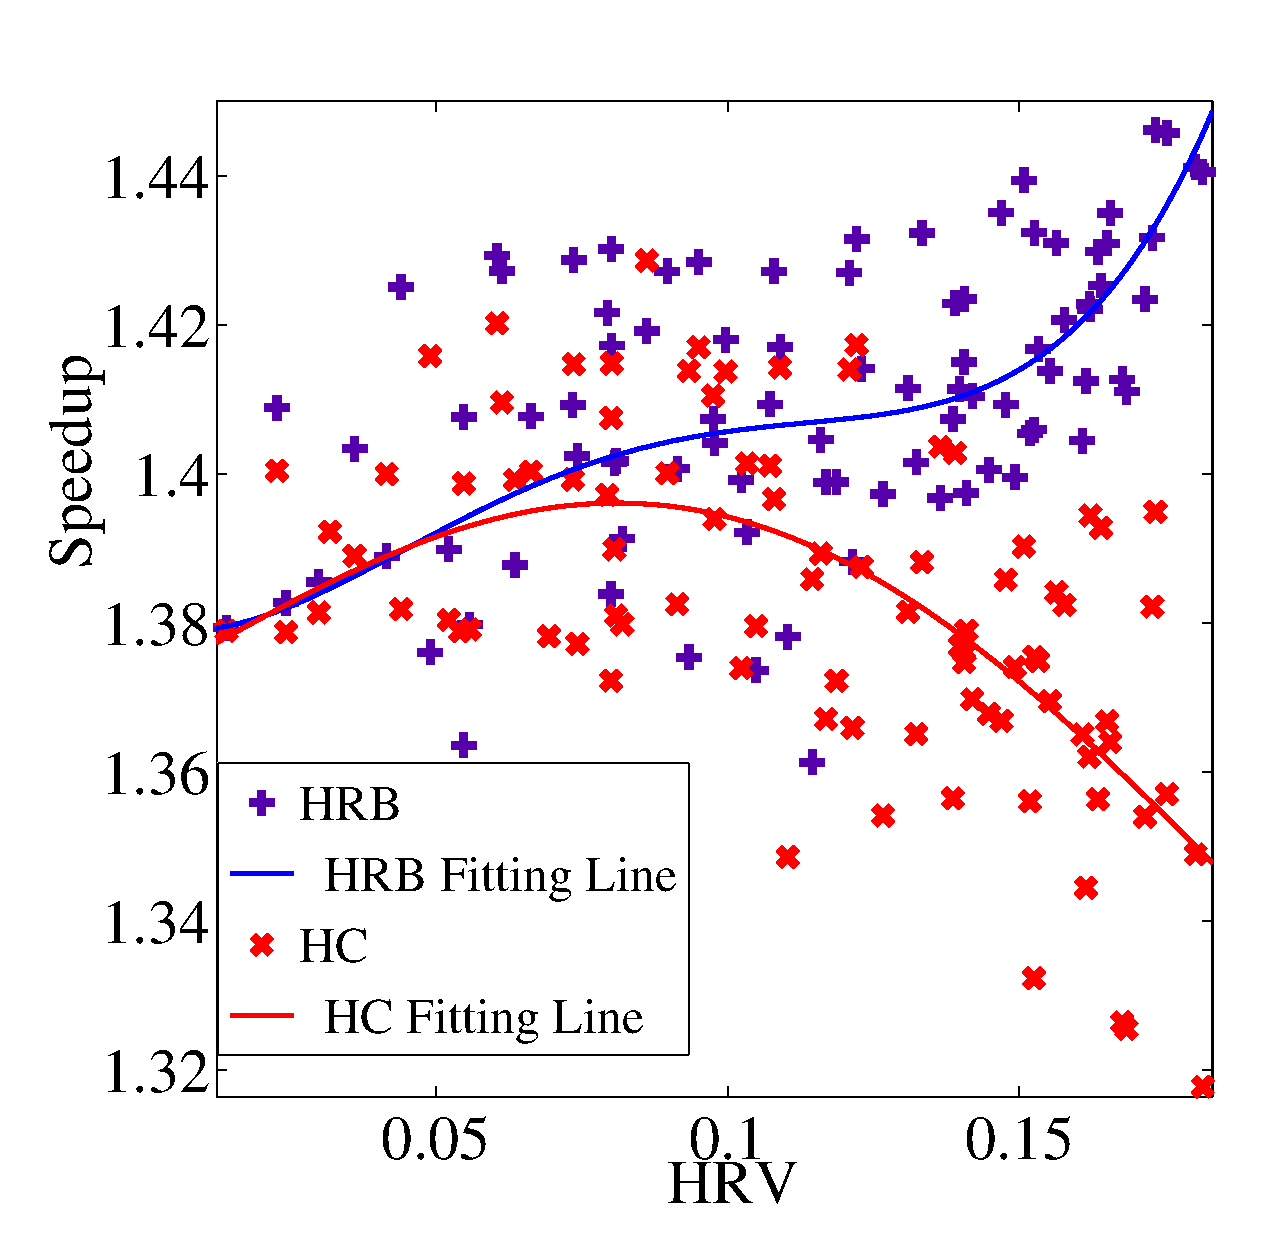
\includegraphics[width=0.9\linewidth]{figures/balance/HRB_figure_2.eps}
  \captionof{figure}{HRB and HC}
  \label{fig:hrb}
\end{minipage}
\end{figure}






To evaluate the dynamic performance of task clustering, we randomly select 20\% of tasks and increase their task runtime by a {\em Ratio\%}. Fig~\ref{fig:shc} shows the Speedup of Horizontal Clustering (HC) with different {\em clustering factor}. We use Speedup of HC in overall runtime compared to the original overall runtime without clustering. The Speedup decreases with the increase of {\em clustering factor}. However, a smaller {\em clustering factor} performs worse when the {\em Ratio} is high. In the rest of this work, we use $clustering~factor=2$ for simplicity. 

\begin{figure}
\centering
  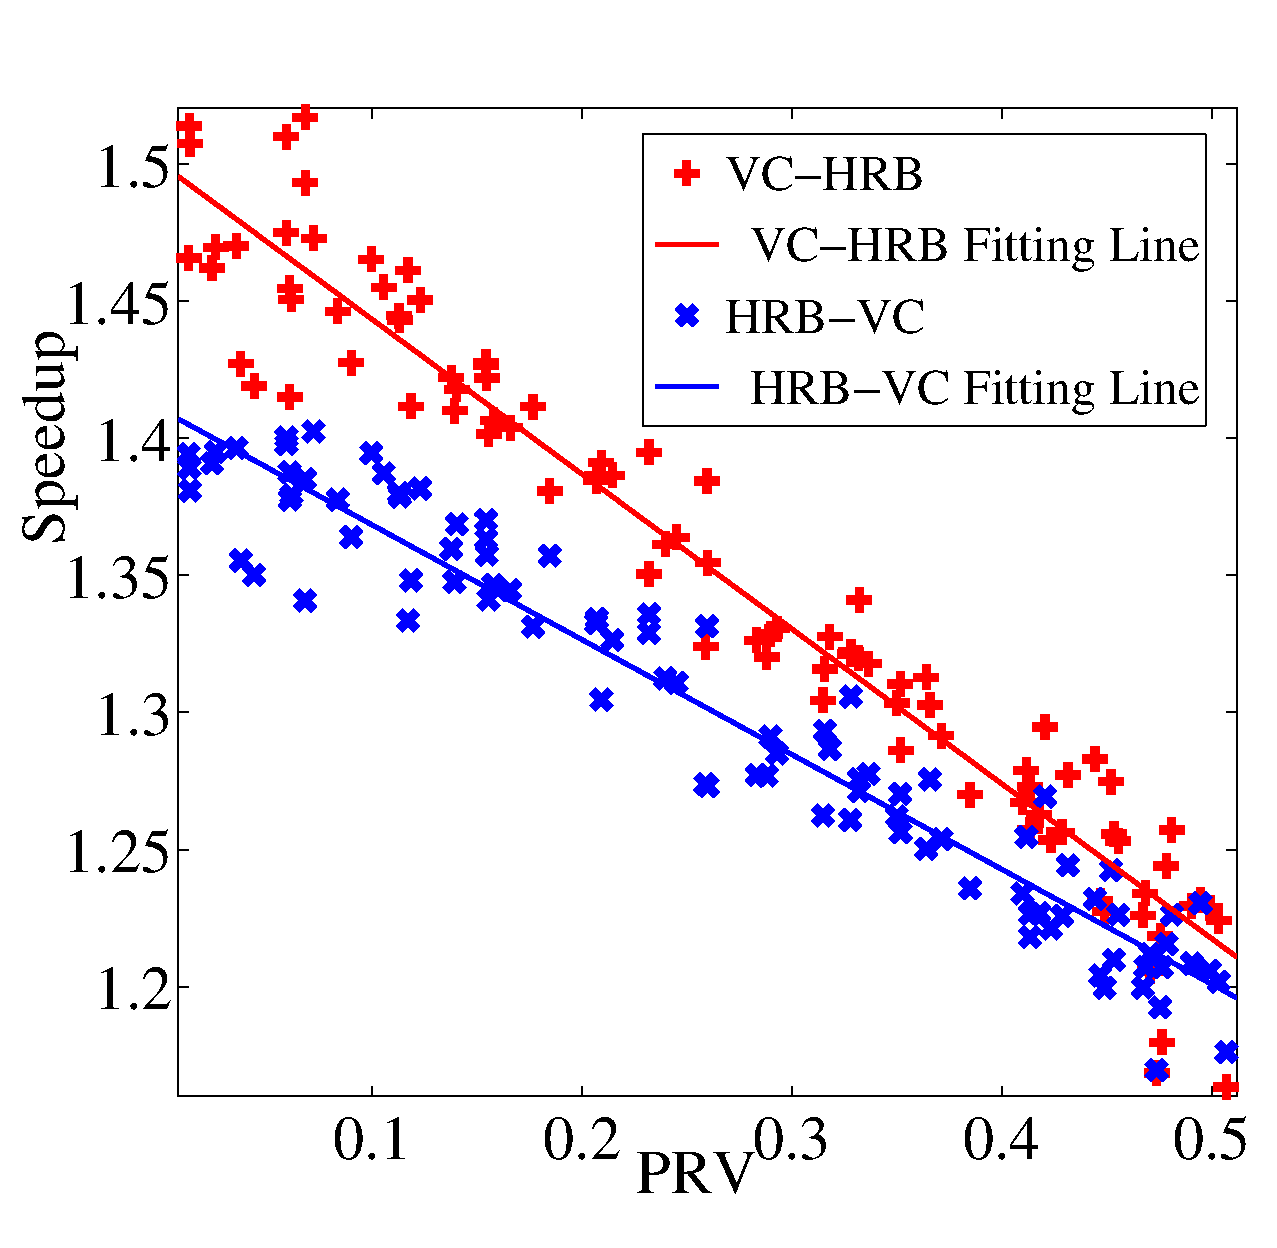
\includegraphics[width=0.5\linewidth]{figures/balance/PRV-VC-figure_2.eps}
  \captionof{figure}{VC-HRB and HRB-VC}
  \label{fig:hvc}
\end{figure}



Fig~\ref{fig:hrb} shows the relationship between the performance of Horizontal Runtime Balancing (HRB) and Horizaontal Runtime Variance ({\em HRV}). We generate 100 workflow instances that have different task runtime distribution (and thus different {\em HRV} and {\em PRV}) and different number of pipelines (and thus different {\em HDV} and {\em HIFV}). Each data point corresponds to one instance. Generally speaking, with the increase of {\em HRV}, the speedup of HRB increases while HC decreases. The reason is HC randomly merges tasks at the same level and is not aware of task runtime. However, the relationship between the Speedup of HRB and {\em HRV} is not a linear increase. The reason is that the Inspiral workflow has multiple levels and a combination of different {\em HRV} per level makes the prediction complicated. 






\begin{figure}
\centering
\begin{tabular}{l|r|r|r|r}
\hline
 & {\em HIFV} & {\em HDV} & {\em HRV} & {\em PRV} \\
\hline
$WF_1$ & 0.0011 & 3140 & 0 & 0\\
$WF_2$ & 0.011 & 11880 & 0  & 0\\
$WF_3$ & 0.015 & 11004 & 0.17 & 0.11\\
\end{tabular}
      \captionof{table}{Workflow Instances}
  \label{tab:3}
\end{figure}

Fig~\ref{fig:hvc} shows the speedup of combining Vertical Clustering (VC) and Horizontal Runtime Balancing (HRB). VC-HRB means we perform VC first and then HRB, and vice versa. The speedup of both VC-HRB and HRB-VC decreases linearly with the increase of {\em PRV}. The reason is there are only two levels of pipelines in the Inspiral workflow and thus the relationship is more explicit. Fig~\ref{fig:hvc} also shows that VC-HRB outperforms HRB-VC. It is because HRB may group the tasks at different pipelines and thus it is difficult for VC to improve the runtime performance further.

\begin{figure}

\centering
\begin{minipage}{.5\textwidth}
  \centering
  \includegraphics[width=1.0\linewidth]{figures/balance//figure3_1.jpg}
  \captionof{figure}{Speedup of $WF_1$}
  \label{fig:tradeoff1}
\end{minipage}%
\begin{minipage}{.5\textwidth}
  \centering
  \includegraphics[width=1.0\linewidth]{figures/balance//figure3_3.jpg}
  \captionof{figure}{Speedup of $WF_2$}
  \label{fig:tradeoff3}
\end{minipage}
\end{figure}

\begin{figure}
\centering
  \includegraphics[width=0.5\linewidth]{figures/balance//figure3_4.jpg}
  \captionof{figure}{Speedup of $WF_3$}
  \label{fig:tradeoff4}
\end{figure}

To evaluate the relative performance of HRB, Horizontal Impact Factor Balancing (HIFB), and Horizontal Distance Balancing (HDB), we select three representative workflow instances ($WF_1$, $WF_2$, $WF_3$ with  metric values shown in Table~\ref{tab:3}) and randomly select 20\% of tasks and increase their task runtime by a {\em Ratio\%}. Comparing Fig~\ref{fig:tradeoff1} and \ref{fig:tradeoff3}, we can see that with the increase of {\em Ratio}, the speedup of all horizontal clustering methods decreases. In contrast, the speedup of Vertical Clustering (VC) is relatively stable because VC never groups tasks in different pipelines. However, the performance of VC is poor compared to horizontal clustering methods when the {\em Ratio} is low. It is because there are still many jobs at the horizontal level and thus the overhead is still significant. 



Also, HIFB and HDB perform better than HRB and HC when the {\em Ratio} is high. The reason is that HDB and HIFB try to avoid merging tasks in different pipelines. However, the difference between HDB, HIFB and HRB is not significant. The reason is that the relative performance is related to Horizontal Impact Factor Variance ({\em HIFV}) and Horizontal Distance Variance ({\em HDV}) but currently we do not have a guideline to increase {\em HIFV} and {\em HDV} significantly and thus we just randomly increase the runtime of a portion of tasks. Moreover, with the increase of all the imbalance metrics, the performance of all the balancing methods decreases as shown in Fig~\ref{fig:tradeoff4}. In conclusion, we believe these imbalance metrics can assist a user or a workflow management system to select one among these balancing methods. If {\em HIFV} or {\em HDV} is high and {\em HRV} is low, we should use HIFB or HDB, otherwise we should use HRB. When all of the metrics are high, none of these balancing methods perform well. When all of them are relatively low, either of these methods can perform well. 
%\begin{figure}{l}[0pt]{6cm}
 % \includegraphics[width=1.0\linewidth]{figures/balance/mapping.jpg}
  %\captionof{figure}{Performance Metric}
  %\label{fig:metric}
%\end{figure}



%\section{Conclusion}

%In this paper, we have proposed four imbalance metrics to evaluate the imbalance problem of a workflow and a series of balancing methods to address this problem.    
In the future, we will explore the difference between HIFV and HDV and the influence of different overheads. We also plan to evaluate more types of workflows. We will also try to dynamically vary the {\em clustering factor} so as to achieve a better performance.


